\chapter{Experiments}
\label{chap:experiments}
\section{Environment}
We developed our experiments environment cluster were listed as table \ref{table:Host}, and created 4 virtual machines in the computer that each of their resource were listed as table \ref{table:Virtual Machine}. We will mount NFS to each virtual machines and test 2 types each of NFS, hard disk, and memory(tmpfs). 
In addition, we also test the difference between \textbf{Direct} method  and \textbf{Track-memory} method as Section \ref{sec:Ticker Strategy}.

\begin{table}[hbtp]
\begin{center}
\begin{tabular}{|c|c|} \hline
CPU & Intel Xeon(R) CPU-E5-2630 v3 @ 2.40GHz x 32 \\ \hline
Memory & 64 GB \\ \hline
Disk & 1.0 TB \\ \hline
OS & Ubuntu 15.10 64 bit \\ \hline
Kernel version & 4.4.4-040404-generic \\ \hline
Docker version & 1.10.3 \\ \hline
Docker Swarm version & 1.2 \\ \hline
Virtual Box version & 5.10.14 \\ \hline
\end{tabular}
\end{center}
\caption{Experiment environment}
\label{table:Host}
\end{table}

\begin{table}[hbtp]
\begin{center}
\begin{tabular}{|c|c|} \hline
CPU & Intel Xeon(R) CPU-E5-2630 v3 @ 2.40GHz x 4 \\ \hline
Memory & 8 GB \\ \hline
Disk & 40 GB \\ \hline
OS & Ubuntu 15.10 64 bit \\ \hline
Kernel version & 4.4.4-040404-generic \\ \hline
Docker version & 1.10.3 \\ \hline
Docker Swarm version & 1.2 \\ \hline
\end{tabular}
\end{center}
\caption{Virtual Machine experiment environment}
\label{table:Virtual Machine}
\end{table}

\section{Container Migration Time}
As shown in Figure \ref{fig:Docker Swarm migration time with remote storage server}, native is a based line of the other kinds of experiment.
We choose Redis\cite{paksula2010persisting} as our migration container, because it uses memory to save its data. Therefore, we can check the correctness of Redis data to make sure container migration is success.

In the beginning, creating the container on another Swarm Nodes is fast for all environments because we assume that they have downloaded their container images from the remote repository, thus, they do not need to transport container images from the other Swarm Nodes.

Next, in \textbf{Track-memory} method, the container has to pre-dump the checkpoint image at the version-group created. After pre-dumping the checkpoint image, dumping checkpoint will track memory different with the pre-dump checkpoint image.
On the other hand, \textbf{Track-memory} method, checkpoint ticker dumps the checkpoint image directly.
The result of total checkpoint time, \textbf{Track-memory} method is longer than the other one, because it has to add pre-dumping checkpoint time and dumping checkpoint time.
Although \textbf{Track-memory} method is longer, but it provides the less frozen time to the container that improves CPU's utilization.

Third, Restoring the container to the container which has already been created in the Swarm Node. Except NFS with memory, they all have nearly performance.

Final, it has big disparity of the delete checkpoint image step at \textbf{Track-memory} method, because it has more image files and directories than the version without pre-dumping version.

After all, the checkpoint and restoration of container in memory is faster than hard disk in NFS.
As result of Figure \ref{fig:Docker Swarm migration time with remote storage server}, NFS with memory has the best performance in this experiment.

\begin{figure}[hbtp]
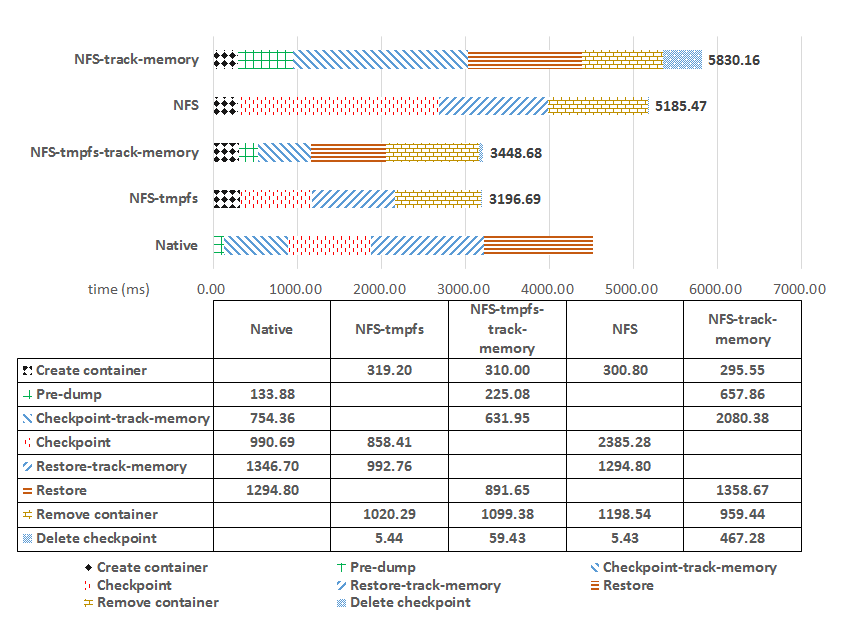
\includegraphics[width=17cm]{figure/migration_time.png}
\caption{Docker Swarm migration with remote storage server}
\label{fig:Docker Swarm migration time with remote storage server}
\end{figure}

\section{The Influence of Container Checkpoint Time on Container Process Time}
\label{sec:CPU Time}
In this experiment, sysbench\cite{kopytov2004sysbench} is used to test performance of process's CPU execution time. Our parameter of sysbench is:
\begin{center}
sysbench --test=cpu --cpu-max-prime=200000 run
\end{center}
It needs to run around 11 minutes in native container without dumping any checkpoint to find the 200000th prime number.

In Figure \ref{fig:Checkpoint Time CPU}, this figure lists every checkpoint time in the experiment environments, also, if remote storage uses the memory to save the checkpoint images, it will get better performance.
In the checkpoint restore rescheduling policy (section \ref{sec:checkpoint restore rescheduling policy}), we set a parameter of checkpoint-ticker period $ T_i $ which will checkpoint repeatedly for every checkpoint-ticker over.

As Figure \ref{fig:Checkpoint Time Influence CPU}, the result of the checkpoint-ticker period $ T_i $ is in direct ratio to the container process execution time.
As these experiment results, the checkpoint-ticker period $ T_i $ has a big influence of container execution time, it is an important parameter in checkpoint restore rescheduling policy that if $ T_i $ is too small, the container will get a bad performance. But if $ T_i $ is too big, whenever Swarm Node fails, the restore container needs to execute the process again. The worst, it might lose some important data. However, no matter the total checkpoint time in \textbf{Track-memory} method, the process's execution time are nearly 
\textbf{Direct} method. This situation shows that the pre-dump checkpoint time has no influence on the process's execution time.

\begin{figure}[hbtp]
\begin{center}
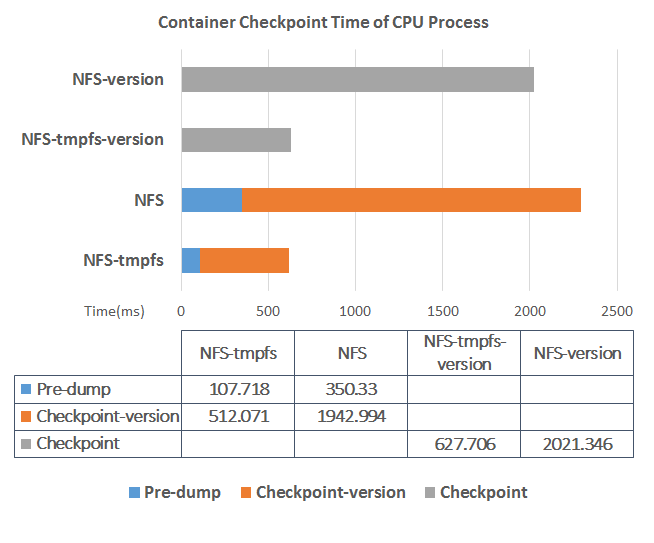
\includegraphics[width=14cm]{figure/cpu_checkpoint_time.png}
\end{center}
\caption{Container checkpoint time of container process time}
\label{fig:Checkpoint Time CPU}
\end{figure}

\begin{figure}[hbtp]
\begin{center}
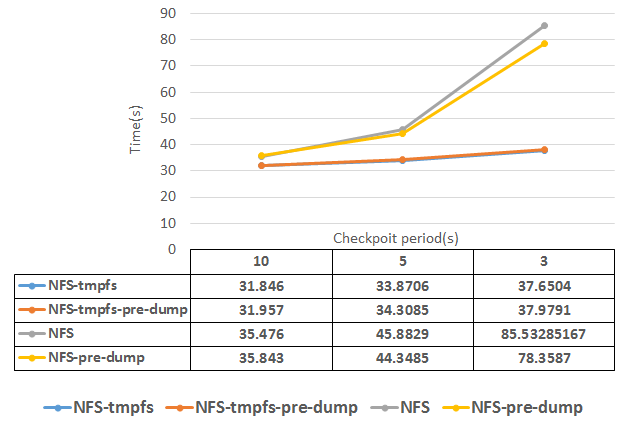
\includegraphics[width=14cm]{figure/cpu_checkpoint_period.png}
\end{center}
\caption{ontainer Checkpoint Time Influence of Container Process Time}
\label{fig:Checkpoint Time Influence CPU}
\end{figure}

\section{The Influence of Many Containers Checkpoint at The Same Time on Container Checkpoint Time}
Figure \ref{fig:many containers} demonstrates the influence of checkpoint time when many containers checkpoint in the same.
As more containers checkpoint in the same time, the more checkpoint time for each container has to take.
In storing in disk case, it almost needs twice times when 4 containers checkpointing in the same time. That's the reason that we implement checkpoint queue to solve this problem.

\begin{figure}[htbp]
\begin{center}
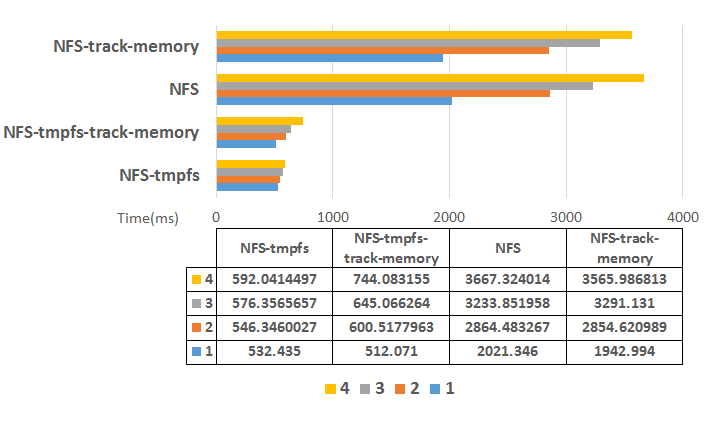
\includegraphics[width=14cm]{figure/many_containers.png}
\end{center}
\caption{Many containers checkpoint in the same time}
\label{fig:many containers}
\end{figure}

\section{Performance of Checkpoint Time and Space}
In this experiment, we checkpoint 50 times the container which executes Redis.  We presume $ VG_i = 5 $, there are 3 scenarios: checkpoint and pre-dump each 5 checkpoint versions, pre-dump once and checkpoint, direct checkpoint every time.  Figure \ref{fig:50_time} shows each scenario checkpoint time.  Table \ref{table:Average Time} demonstrates that checkpoint and pre-dump each 5 checkpoint versions is faster than direct checkpoint each time about 15\% when used hard disk as remote storage.  Figure \ref{fig:50_space} shows the disk usage.  Checkpoint and pre-dump each 5 checkpoint versions(1 pre-dump and 5 checkpoint) saves about 200\% than direct checkpoint each time(5 checkpoint) when container has 5 version of checkpoint.

\begin{figure}[htbp]
\begin{center}
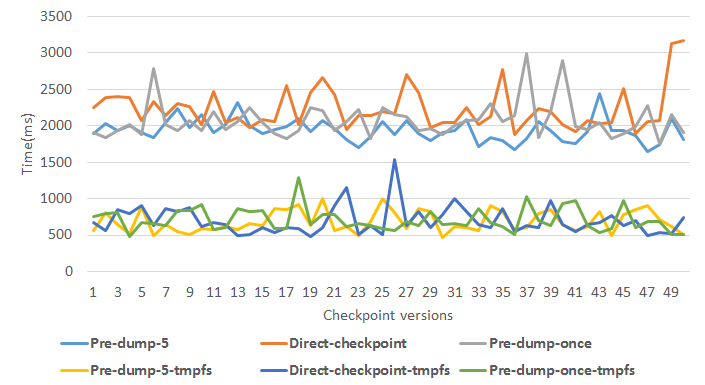
\includegraphics[width=14cm]{figure/50_time.png}
\end{center}
\caption{Disk space}
\label{fig:50_time}
\end{figure}

\begin{table}[htbp]
\centering
\begin{tabular}{|l|l|l|l|}
\hline
          & Pre-dump-5 & Pre-dump-once & Direct-checkpoint \\ \hline
Hard disk & 1938.212   & 2071.731      & 2233.558          \\ \hline
Tmpfs     & 685.7929   & 711.0002      & 700.2387          \\ \hline
\end{tabular}
\caption{Average Time}
\label{table:Average Time}
\end{table}

\begin{figure}[htbp]
\begin{center}
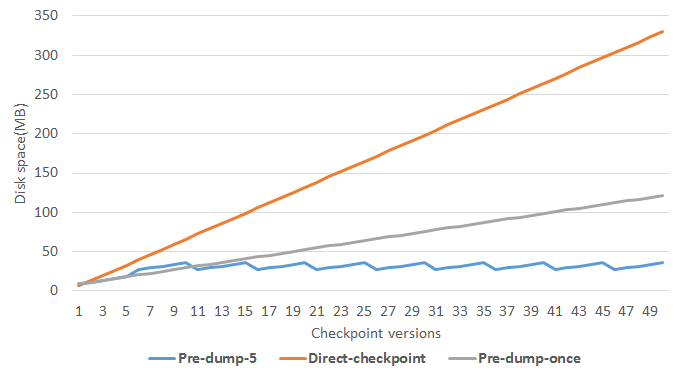
\includegraphics[width=14cm]{figure/50_space.png}
\end{center}
\caption{Checkpoint time}
\label{fig:50_space}
\end{figure}